\section{Results}\label{sec:results}
\subsection{Atomic recovery and spectral leakage}
Table~\ref{tab:primary} reports the 36 signal-present atomic test problems. RAI-S reduces mean leakage from 5.166\% to 1.728\%, and DOME-S from 3.857\% to 1.728\%. The clean external prediction error decreases from 0.2870 to 0.2330 for RAI and from 0.2591 to 0.2330 for DOME. Binned shape loss decreases from 0.1523 to 0.1094 and from 0.1393 to 0.1094, respectively. These are paired changes on the same observations and masks.

\begin{table}[htbp]
\caption{New atomic test: 36 signal-present problems, excluding null and broad-distribution controls. Leakage and unmatched mass are percentages. $E_U$ is clean external RMSE divided by $\sigma$; $W_{1,h}$ is the binned log-diffusion shape score. A correct count is weaker than recovery of both order and rates.}\label{tab:primary}
\begin{adjustwidth}{-\extralength}{0cm}\centering\small
\begin{tabular}{lrrrrrr}\toprule
Method & Correct order & Order and rates & Leakage & Unmatched mass & $E_U$ & $W_{1,h}$\\\midrule
RAI & 17/36 & 17/36 & 5.166 & 6.774 & 0.2870 & 0.1523 \\
RAI-S & 25/36 & 23/36 & 1.728 & 7.257 & 0.2330 & 0.1094 \\
DOME & 26/36 & 22/36 & 3.857 & 7.019 & 0.2591 & 0.1393 \\
DOME-S & 25/36 & 23/36 & 1.728 & 7.257 & 0.2330 & 0.1094 \\
\bottomrule\end{tabular}

\end{adjustwidth}
\end{table}

The favorable averages do not hold for every endpoint. Unmatched estimated mass increases from 6.774\% to 7.257\% for RAI and from 7.019\% to 7.257\% for DOME. RAI's correct-order count rises from 17/36 to 25/36, but DOME's falls from 26/36 to 25/36. The stricter order-and-rates count improves from 17/36 to 23/36 and from 22/36 to 23/36. Thus the strongest common conclusion is improved spectral assignment and prediction, not uniformly improved component counting.

For RAI, the mean leakage change is $-3.438$ percentage points, with a descriptive 95\% paired bootstrap interval $[-5.282,-1.926]$. For DOME the change is $-2.129$ points, with interval $[-3.155,-1.268]$. The corresponding clean prediction changes are $-0.0540$ [$-0.0800,-0.0325$] and $-0.0261$ [$-0.0338,-0.0181$]. These intervals summarize the saved 36-case panel under the stated resampling convention; they do not adjust for multiple reported endpoints or establish external experimental performance.

RAI-S and DOME-S yield effectively identical primary summaries to the displayed precision. Their common post-proposal objective, support rule, and refinement can erase differences between proposal paths. These outcomes support the shared selection procedure and give no evidence that two independent improvements have been discovered.

\subsection{Scenario-level failures and a DOSY illustration}
Figure~\ref{fig:recovery} separates ordinary mixtures from difficult identification regimes. Both screened methods recover order and all rates in all six one-, two-, and three-separated-component cases. In close-rate cases they recover the correct order in 5/6 problems, but all rates in only 4/6. For proportional spectra they recover neither the full three-rate structure nor the correct order in any of six cases. The original DOME recovers the correct order in one of these cases, so the screened version has a visible regression.

In the weak family, the correct order is selected in 2/6 cases, but the weakest rate is matched in only 1/6; neither original method matches it in these six cases. In the one matched screened case, approximately 72\% of the true minority spectral mass lies within the retained allowed support. The support metric is a recall of permitted frequencies, not a claim of unbiased amplitude recovery. These results leave weak-species detection unresolved.

\begin{figure}[htbp]\centering
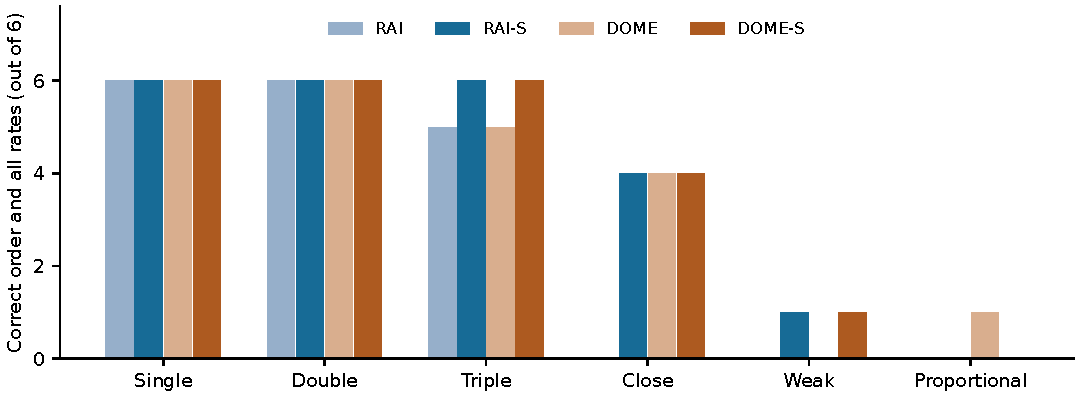
\includegraphics[width=\linewidth]{figures/recovery.pdf}
\caption{Recovery of both order and all rates by scenario in the new atomic test. Every bar has six independently generated problems. Matching uses a log-rate tolerance of 0.25. Narrow output bands and correct order alone do not imply successful localization.}\label{fig:recovery}
\end{figure}

\begin{figure}[p]
\begin{adjustwidth}{-\extralength}{0cm}\centering
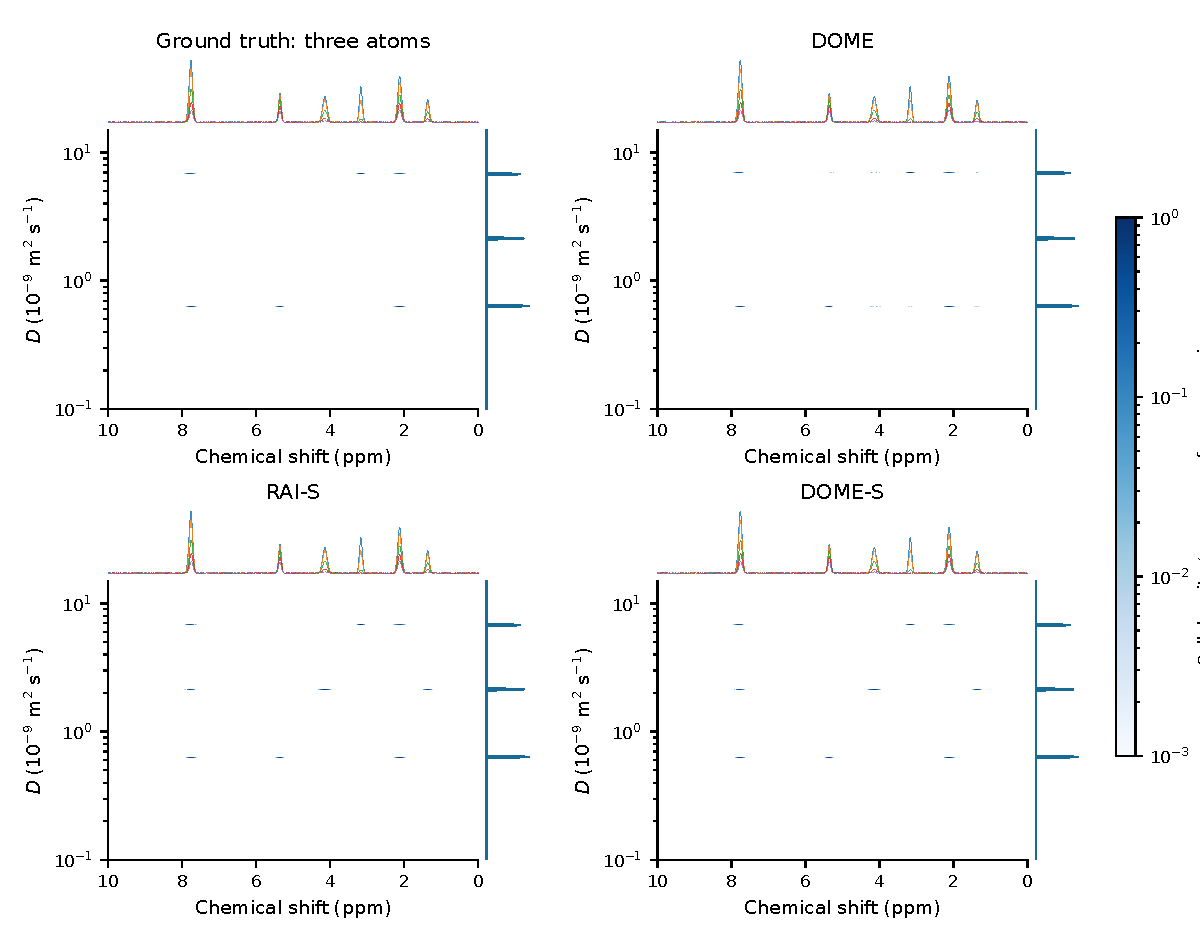
\includegraphics[width=\fulllength,height=.77\textheight,keepaspectratio]{figures/dosy_discrete.pdf}
\caption{Saved independent test problem 18, with three true atomic rates and SNR 200. The complete reference is shown alongside DOME and the two support-selected outputs. All panels use the same selected frequencies, 256-bin mass-to-density display, and common absolute reference maximum; values below 0.1\% of that maximum are not colored. The top traces show measured attenuation spectra. Side projections have separate horizontal scales. The display creates finite-width cells for atoms; it is not a recovered continuous width. Quantitative results use the unthresholded saved outputs.}\label{fig:dosyatomic}
\end{adjustwidth}
\end{figure}

Figure~\ref{fig:dosyatomic} provides one fixed illustration, rather than selecting a new representative after ranking the test outputs. The ground truth is displayed explicitly. Correlation is used through common rates and component-specific spectral amplitudes; it is not an assumption that every frequency has the same decay. The color threshold is a plotting convention applied to every panel and has no role in model order or support estimation.

\subsection{Null controls, broad distributions, and transfer}
All four atomic methods select the null model in all six noise-only controls. This observed count is not a guarantee of a population false-positive rate. On the six broad controls, the screened methods have clean prediction error 0.2382, compared with 0.3664 for RAI and 0.2837 for DOME. Their binned shape score is 0.1638, compared with 0.2686 and 0.1972. An atom model nevertheless cannot reproduce nonzero distributional width exactly. Counting its fitted rates against the number of generating broad profiles is a descriptive center-count comparison, not a valid literal atom-recovery claim.

On the 24 archived finite-width problems, leakage decreases from 1.245\% to 0.082\% for both native paths. Clean prediction error changes from 0.2650 to 0.2329 for RAI and from 0.2492 to 0.2329 for DOME. The selected-order count agrees with the number of generating profiles in 19/24 screened fits versus 18/24 native fits, while the stricter matching count remains 18/24. Transfer performance is encouraging for spectral assignment, but the differing true measure class prevents pooling it with the atomic test.

\begin{figure}[p]
\begin{adjustwidth}{-\extralength}{0cm}\centering
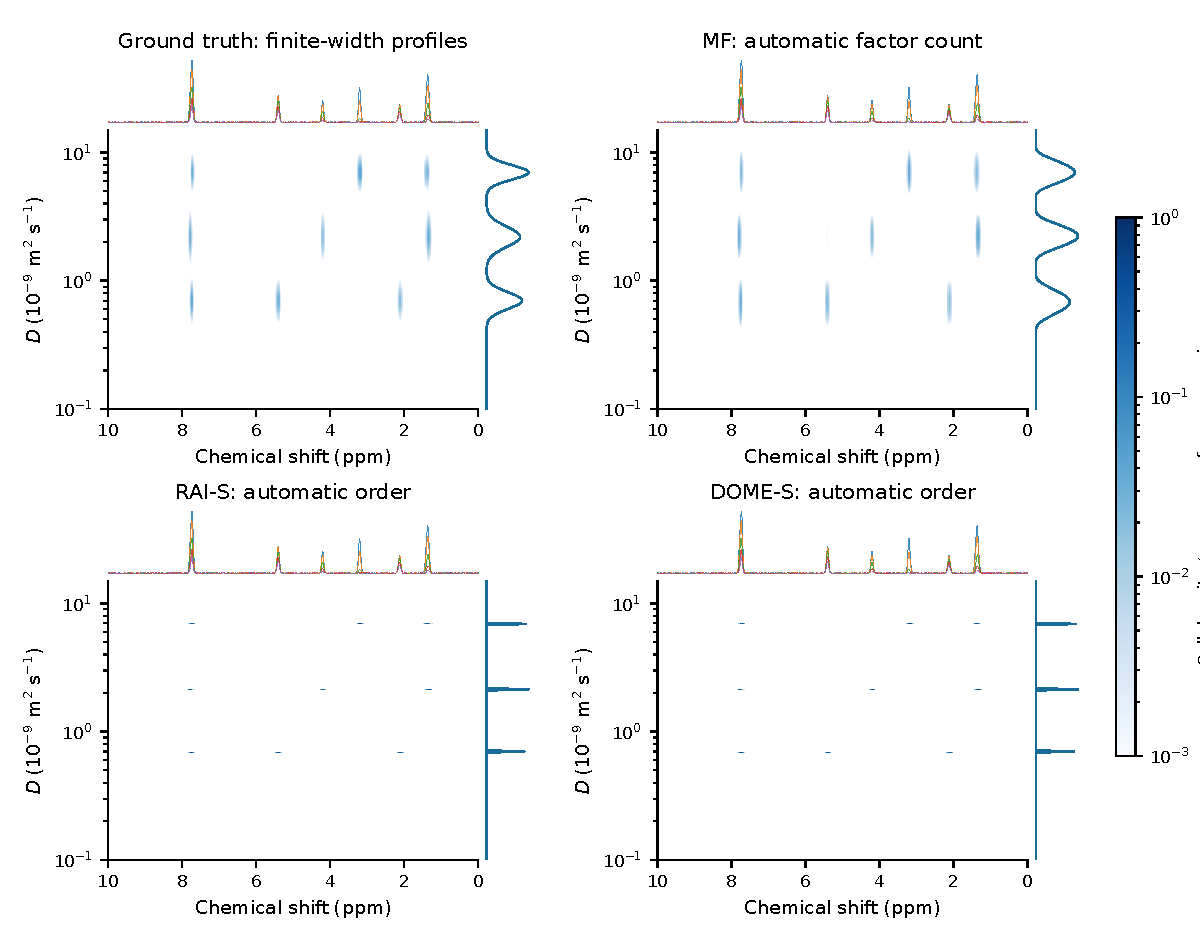
\includegraphics[width=\fulllength,height=.77\textheight,keepaspectratio]{figures/dosy_continuous.pdf}
\caption{Archived problem \texttt{r3\_snr200\_rep1}: three finite-width lognormal diffusion profiles, SNR 200, and 120 selected frequencies of 1024. Ground truth, the unchanged automatic MF reference, RAI-S, and DOME-S are shown. MF uses its original masses and original cell edges without remapping. Its factor count and the atomic methods' order are selected automatically but have different meanings. The common reference maximum is 63.34986357 in the saved cell-density units, with a 0.1\% display floor. Side projections are separately scaled. Fitted atoms occupy individual export cells and do not estimate the true widths.}\label{fig:dosycontinuous}
\end{adjustwidth}
\end{figure}

Figure~\ref{fig:dosycontinuous} retains the existing MF reconstruction and its native grid. For this case, the native atomic leakage of approximately 1.975\% decreases to 0.279\% after support selection, with three selected rates. The MF result is used to display the distinction between distributional factorization and atomic inference. It was not recomputed for this manuscript, and the figure is not a new all-method performance ranking. No conclusion about polymer molecular weights is drawn without a separate calibration and experimental analysis.

\subsection{Neural policy ablation}
Table~\ref{tab:net} reports the policy comparison. On 24 new test problems the relative change in mean binned shape score is approximately 0.041\%, with mean paired difference $-0.000111$ and bootstrap interval $[-0.001356,0.001105]$. The clean-error interval also includes zero. On the archived transfer panel, the shape score improves by approximately 1.48\%, but this does not establish an advantage on the new test. One fit per policy in the archived panel fails its numerical convergence criterion; both outputs remain in the reported averages.

\begin{table}[htbp]\centering
\caption{RAI-Net policy ablation on its predefined panels. These are distributional methods, so no chemical order-recovery count is assigned. All saved outcomes, including the two numerical failures, enter the averages.}\label{tab:net}
\begin{tabular}{llrrr}\toprule
Panel & Policy & $W_{1,h}$ & $E_U$ & Numerical success\\\midrule
New test, $n=24$ & Original & 0.272268 & 0.307991 & 24/24\\
 & Retrained & 0.272157 & 0.307921 & 24/24\\
Archived, $n=24$ & Original & 0.204769 & 0.326401 & 23/24\\
 & Retrained & 0.201739 & 0.326324 & 23/24\\\bottomrule
\end{tabular}
\end{table}

The new neural panel includes atomic, broad, and null cases, with zero shape-score contributions for nulls under the archived bookkeeping convention. Its averages therefore do not share the population of Table~\ref{tab:primary}. The policy ranks adaptive actions within an existing numerical procedure. It neither adds observations nor certifies the chemical support. These data do not support promoting the retrained policy as a superior substitute for the support-selected atomic estimator, and the two are not compared as if they shared the same output class.

\subsection{Numerical and provenance checks}
The archived audit verifies 144 support-selected fits across the new test and transfer banks. Their maximum relative amplitude KKT residual is $1.12\times10^{-15}$; the maximum normalized projected log-rate residual is $1.34\times10^{-7}$. Four poor-precision flags and four atomic-model-mismatch flags remain visible. The 100-column MATLAB NNLS comparison has relative prediction discrepancy $4.62\times10^{-17}$. Five targeted numerical tests pass. These figures are compatibility and numerical checks, not confidence bounds for chemical recovery.

An earlier clean extraction of the reproducibility bundle reproduced a selected prediction exactly. A later correction restored the original MF plotting grid and color floor without changing its numerical result or the support-selection core. The current manuscript hashes its input files and regenerates tables and figures from saved outputs. The MF array hash remains unchanged. Appendix~\ref{app:repro} specifies the replay and refitting scopes of the public release and the exploratory work retained in earlier archives.
